		% \begin{table}[!h]
		% 	\caption{Overview: Scene Classification Layers (SCL)}
		% 	\label{tab:satelite/scl_classes}
		% 	\center
		% 	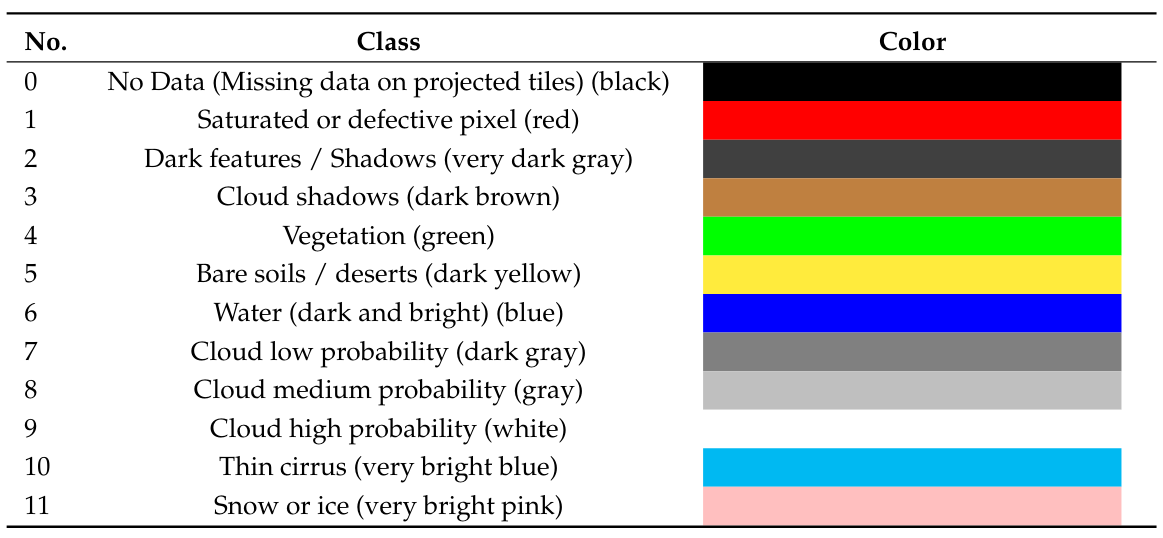
\includegraphics[width=0.8\textwidth]{satelite/scl_classes.png}
		% \end{table}
		
		\begin{table}[h]
			\caption{Overview: Scene Classification Layers (SCL)}
			\label{tab:satelite/scl_classes}
			\centering
			\small
			\begin{tblr}{
			  colspec = {p{0.05\linewidth} p{0.03\linewidth} p{0.3\linewidth} p{0.05\linewidth} p{0.03\linewidth} p{0.3\linewidth} },
			%   row{2} = {SCL3color},
			%   column{3} = {teal7},
			  cell{2}{1} = {SCL0color},
			  cell{3}{1} = {SCL1color},
			  cell{4}{1} = {SCL2color},
			  cell{5}{1} = {SCL3color},
			  cell{6}{1} = {SCL4color},
			  cell{7}{1} = {SCL5color},
			  cell{2}{4} = {SCL6color},
			  cell{3}{4} = {SCL7color},
			  cell{4}{4} = {SCL8color},
			  cell{5}{4} = {SCL9color},
			  cell{6}{4} = {SCL10color},
			  cell{7}{4} = {SCL11color},
			}
			% \toprule % not working :8
			\hline
			Color & No. & Class & Color & No. & Class \\
			\hline
			& 0: & Missing Data 	& & 6: &  Water\\	 
			& 1: & Saturated or defective pixel 	& & 7: &  Cloud low probability\\
			& 2: & Dark features / Shadows 	& & 8: &  Cloud medium probability\\
			& 3: & Cloud shadows 	& & 9: &  Cloud high probability\\
			& 4: & Vegetation 	& & 10: &  Thin cirrus cloud\\
			& 5: & Bare soils 	& & 11: &  Snow or ice\\
			  \hline
			%   \bottomrule
			\end{tblr}
		  \end{table}


	% 0: "#000000",  Missing Data
	% 1: "#ff0000",	 Saturated or defective pixel
	% 2: "#404040",  Dark features / Shadows
	% 3: "#bf8144",  Cloud shadows
	% 4: "#00ff3c",  Vegetation
	% 5: "#ffed50",  Bare soils
	% 6: "#0d00fa",  Water
	% 7: "#808080",  Cloud low probability
	% 8: "#bfbfbf",  Cloud medium probability
	% 9: "#eeeeee",  Cloud high probability
	% 10: "#0bb8f0", Thin cirrus cloud
	% 11: "#ffbfbf", Snow or ice
